\section{Introduction}
\label{sec:introduction}
\subsection{Background}
	There are many robots created to improve quality of our life, one of the robot example is Roomba. Roomba is a series of autonomous robotic vacuum cleaners sold by iRobot. Roomba features a set of basic sensors that enable it perform its tasks. For instance, the Roomba is able to change direction on encountering obstacles, to detect dirty spots on the floor, and to sense steep drops to keep it from falling down stairs. \cite{wiki:Roomba} 
	\begin{figure}[ht]
	\centering
	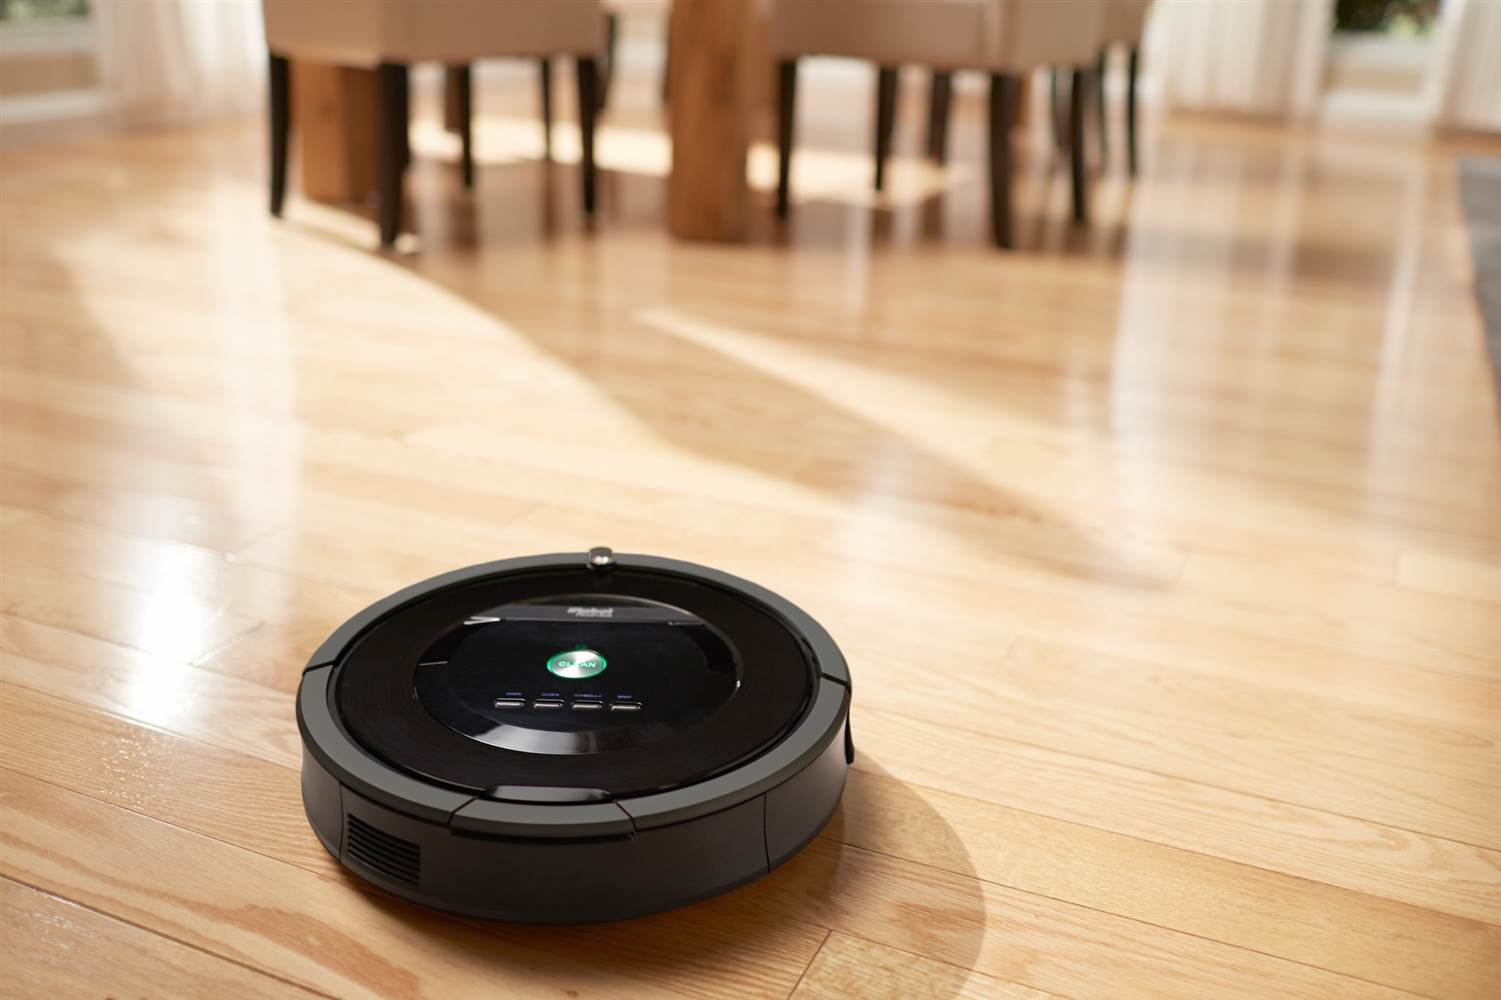
\includegraphics[width=0.45\textwidth]{roomba}
	\caption{Roomba}
	%\label{fig1}
	\end{figure}
	\par
	

	However, when multiple Roomba robots are used, it is hard for them to avoid collision and communicate with each other, so the AI of robots that can localize themselves can make a great contribution. What's more, we may want to easily find a specific room location even when we are not familiar with the place.  We can navigate our outdoor position with GPS, but it is hard for us to know our indoor position with our smart devices. All of these problems lead to the topic on how to implement the localization of the robots.
\par
	In terms of localization, our method is to find direction firstly and measure the distance along with the direction. There are several algorithms of direction of arrival, we choose to use MUSIC algorithm , stands for MUiltiple SIgnal Classification, one of the high resolution subspace DOA algorithms, which gives the estimation of number of signals arrived, hence their direction of arrival. Compare with other algorithm, it is able to estimate frequencies with accuracy higher than one sample, because its estimation function can be evaluated for any frequency. This is a form of superresolution. MUSIC estimates the frequency content of a signal or autocorrelation matrix using an eigenspace method. This method assumes that a signal, $x(n)$, consists of $p$ complex exponentials in the presence of Gaussian white noise. Given an $M \times M$ autocorrelation matrix, $\mathbf{R}_x$, if the eigenvalues are sorted in decreasing order, the eigenvectors corresponding to the p largest eigenvalues (i.e. directions of largest variability) span the signal subspace. The remaining $M-p$ eigenvectors span the orthogonal space, where there is only noise. Note that for $M = p + 1$, MUSIC is identical to Pisarenko harmonic decomposition. The general idea is to use averaging to improve the performance of the Pisarenko estimator. The equation of MUSIC will be described later. Figure 1 shows the MUSIC algorithm. \cite{wiki:MUSIC} \cite{music}
	\begin{figure}[ht]
	\centering
	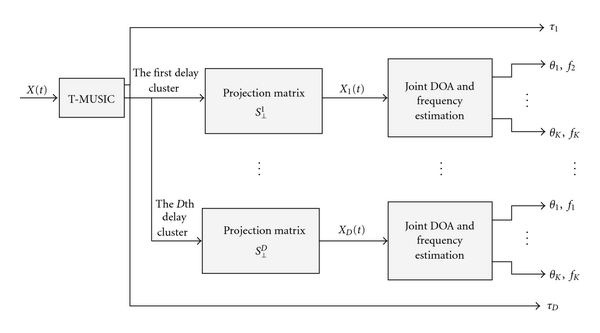
\includegraphics[width=0.45\textwidth]{music}
	\caption{MUSIC algorithm chart}
	%\label{fig1}
	\end{figure}
	
\par
	After the procedure of DOA, we will estimate distance based on path loss with noise of Rayleigh fading and Gaussian white noise. Path loss is the reduction in power density of an electromagnetic wave as it propagates through space. This term is commonly used in wireless communications and signal propagation. Although path loss may be due to many effects, such as free-space loss, refraction, diffraction, reflection, aperture-medium coupling loss, and absorption, we decide to use simple version of pass loss equation without considering so many effects, which is commonly used and called free space propagation. The simplified equation will be described later. Figure 2 shows the characteristics of wireless channel related to path loss vs. distance. \cite{elsayed} \cite{wiki:Pathloss} 
	\begin{figure}[ht]
	\centering
	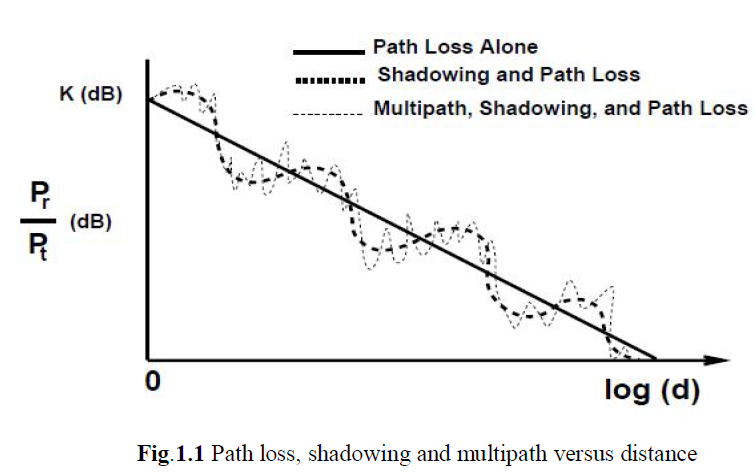
\includegraphics[width=0.45\textwidth]{pathloss}
	\caption{Path loss vs. distance}
	%\label{fig1}
	\end{figure}
\par
	In terms of noise simulation, we decide to use the effect of Rayleigh fading,a statistical model for the effect of a propagation environment on a radio signal, such as that used by wireless devices. Rayleigh fading models assume that the magnitude of a signal that has passed through such a transmission medium (also called a communications channel) will vary randomly, or fade, according to a Rayleigh distribution — the radial component of the sum of two uncorrelated Gaussian random variables. Rayleigh fading is most applicable when there is no dominant propagation along a line of sight between the transmitter and receiver. In addition to Rayleigh fading noise, we also add Gaussian white noise, which is also known as normal distribution white noise. It is very commonly used in signal processing because of the central limit theorem, it states that averages of random variables independently drawn from independent distributions converge in distribution to the normal, that is, become normally distributed when the number of random variables is sufficiently large.  A random variable with a Gaussian distribution is said to be normally distributed and is called a normal deviate if mean of the distribution is 0 and its standard deviation is 1. \cite{wiki:Rayleighfading} \cite{wiki:Normaldistribution} \cite{white_noise}
	\begin{figure}[ht]
	\centering
	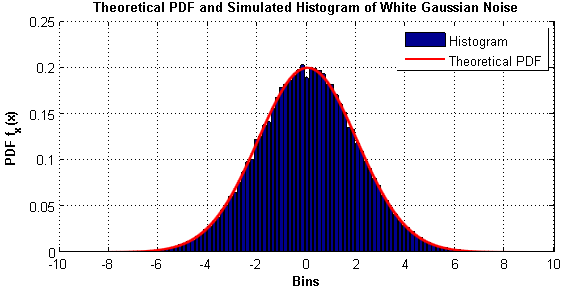
\includegraphics[width=0.45\textwidth]{white_noise}
	\caption{Distribution of White Noise}
	%\label{fig1}
	\end{figure}


\subsection{Related Work}
Daniel B. Faria, published a report, "Modeling Signal Attenuation in IEEE 802.11 Wireless LANs", presented experimental data that validates the use of the log-distance model both inside and outside a standard office building. In his project, path loss models are used to approximate signal attenuation as a function of the distance between transmitters and receivers, being an important building block for both research and industry efforts. Based on experiments with off-the-shelf 802.11 hardware, they had shown that the log-distance path loss model with log-normal shadowing can be used to estimate signal attenuation both inside and outside an office building with moderate accuracy. As a result, we will not consider the environment effect of indoor and outdoor in our project. \cite{faria2005modeling}
\par
R.C. Smith and P. Cheeseman in 1986, and the research group of Hugh F. Durrant-Whyte in the early 1990s, proposed an algorithm called simultaneous localization and mapping (SLAM),which is the computational problem of constructing or updating a map of an unknown environment while simultaneously keeping track of an agent's location within it. \cite{wiki:SLAM}
\par
Leonard, J.J. and Durrant-Whyte, H.F., proposed a report of mobile robot localization by tracking geometric beacons in 1991. The algorithm is based on an extended Kalman filter that utilizes matches between observed geometric beacons and an a priori map of beacon locations. Two implementations of this navigation algorithm, both of which use sonar, are described. The first implementation uses a simple vehicle with point kinematics equipped with a single rotating sonar. The second implementation uses a `Robuter' mobile robot and six static sonar transducers to provide localization information while the vehicle moves at typical speeds of 30 cm/s. \cite{88147}
%\begin{figure}[h]
%\centering
%\includegraphics[width=0.8\linewidth]{img/img1}
%\caption{3D terrain surface}
%\label{fig4}
%\end{figure} 

%application \cite{Sichitiu, Musolesi2009}
%realistic \cite{Jardosh2003}
%general survey \cite{Camp2002,Bai2004}
%group \cite{Hong1999}
%probability \cite{Mohimani2009}